\documentclass[10pt,a4paper]{article}
\usepackage[utf8]{inputenc}
\usepackage{amsmath}
\usepackage{amsfonts}	%Gestion dans les environnements mathématiques.
\usepackage{amssymb}
\usepackage{bbm}		%Gestion des caractères pour les ensembles (N, Z, Q, R, C)
\usepackage{graphicx} 	%Gestion des images.
\usepackage{array}		%Gestion spécifique pour les tableaux.
						%Paramètres de placement dans les cellules: m, p, b. 
						%Avec dimensionnement de la colonne: m{2cm}.
\usepackage{multicol}	%Gère la mise en colonnes du texte.
\usepackage[english]{babel}  %Pour les fonctionnalités en français (language).
%\usepackage[T1]{fontenc}    %Pour les fonctionnalités en français (font),
							%parmamètre par défaut: OT1.
\usepackage{fancyhdr}	%Gère la personnalisation des headers.
\usepackage{geometry}
\usepackage{marginnote}	%Gère la création de notes en marge du texte.
\usepackage{adjustbox}	%Options additionnelles de placement de l'image 
						%(left, right, center, outer and inner)
%-----------------------------------------------------------------------------
\title{Quaternions Theory}
\author{Lucas Wälti}
\date{\today}
%-----------------------------------------------------------------------------
\pagestyle{fancy} 	%Types de headers standards: empty, plain (default),
					%							 headings, myheadings, fancy.
\fancyhf{}			%Clear le header et footer par défaut.
\rhead{Quaternion Theory}
\lhead{}	%Texte à droite, gauche et au centre du header.
\chead{}
\rfoot{}
\lfoot{}
\cfoot{Page \thepage}			%Texte du footer (ici: numéro de page).

\renewcommand{\headrulewidth}{0.5pt}
\renewcommand{\footrulewidth}{0pt}	%Lignes horizontales de séparation.
%-----------------------------------------------------------------------------
\begin{document}
\maketitle
\thispagestyle{empty}	%Supprime le header et le footer pour cette page. 
\large
\section{Quaternion Manipulations}
A quaternion is given as
$$
q = (w,x,y,z) \longleftrightarrow  w + xi + yj +zk
$$
where $w$ is the \emph{scalar} and $(x,y,z)$ is the $vector$. 
The following rule generates all properties of the quaternions: 
$$
\boxed{
i^2 = j^2 = k^2 = ijk = -1
}
$$
which implies following multiplication properties: 
\begin{center}
\begin{tabular}{c|ccc}
$\cdot\Rsh$ & i & j & k \\ 
\hline 
i & -1 & k & -j \\ 
j & -k & -1 & i \\ 
k & j & -i & -1 \\ 
\end{tabular} 
\end{center}

\subsection{Addition}
$$
q_1 + q_2 = (a,b,c,d) + (e,f,g,h) = (a+e,b+f,c+g,d+h)
$$
\subsection{Multiplication}
$$
q_1 = a + bi +cj + dk
$$
$$
q_2 = e + fi + gj + hk
$$
The multiplication is then:
\begin{equation*}
\begin{split}
q_1q_2 =  ae + afi + agj + ahk +\\ 
bei + bfi^2 + bgij + bhik +\\
cej + cfji + cgj^2 + chjk +\\
dek + dfki + dgkj + dhk^2 
\end{split}
\end{equation*}
Which results in:
\begin{equation*}
\boxed{
\begin{split}
q_1q_2 = (ae - bf - cg - dh, \\
af + be + ch - dg, \\
ag - bh + ce + df, \\
ah + bg - cf + de)
\end{split}
}
\end{equation*}
Note that $q_1q_2 \neq q_2q_1$. 

\subsubsection{Quaternions seen as Matrices}
We can rearrange the multiplication like this:
\begin{equation*}
\begin{split}
q_1q_2 = (a,b,c,d)(e,f,g,h) = (ae - bf - cg - dh, \\
be + af - dg + ch, \\
ce + df + ag - bh, \\
de - cf + bg + ah)
\end{split}
\end{equation*}
Which we rewrite as: 
$$
q_1q_2 = 
\left[ {\begin{array}{cccc} 
	a & -b & -c & -d \\
	b & a & -d & c \\
	c & d & a & -b \\
	d & -c & b & a 
\end{array} } \right]
\cdot
\left[ {\begin{array}{c} 
	e \\
	f \\
	g \\
	h
\end{array} } \right]
$$
This can be applied to:
$$
1 = (1,0,0,0) \longrightarrow 
\left[ {\begin{array}{cccc} 
	1 & 0 & 0 & 0 \\
	0 & 1 & 0 & 0 \\
	0 & 0 & 1 & 0 \\
	0 & 0 & 0 & 1
\end{array} } \right]
= 1
$$
$$
i = (0,1,0,0) \longrightarrow 
\left[ {\begin{array}{cccc} 
	0 & -1 & 0 & 0 \\
	1 & 0 & 0 & 0 \\
	0 & 0 & 0 & -1 \\
	0 & 0 & 1 & 0
\end{array} } \right]
= i
$$
$$
j = (0,0,1,0) \longrightarrow 
\left[ {\begin{array}{cccc} 
	0 & 0 & -1 & 0 \\
	0 & 0 & 0 & 1 \\
	1 & 0 & 0 & 0 \\
	0 & -1 & 0 & 0
\end{array} } \right]
= j
$$
$$
k = (0,0,0,1) \longrightarrow 
\left[ {\begin{array}{cccc} 
	0 & 0 & 0 & -1 \\
	0 & 0 & -1 & 0 \\
	0 & 1 & 0 & 0 \\
	1 & 0 & 0 & 0
\end{array} } \right]
= k
$$

\subsection{Extracting the Dot and Cross Products}
Let us consider the multiplication with the following notation: 
$$
q_1q_2 = (w_1,\vec{v_1})(w_2,\vec{v_2})
$$
If we compare it to the first notation in section 1.2.1, we observe that:
$$
\boxed{
q_1q_2 = (w_1w_2 - \vec{v_1}\cdot\vec{v_2}, w_2\vec{v_1} + w_1\vec{v_2} + \vec{v_1}\wedge\vec{v_2})
}
$$
Let us build the following quaternions:
$$
v_1v_2 = (0,\vec{v}_1)(0,\vec{v}_2) = (-\vec{v}_1\cdot\vec{v}_2, \vec{v}_1\wedge\vec{v}_2)
$$
We can see that:
$$
v_1v_2 = (-\vec{v}_1\cdot\vec{v}_2, \vec{v}_1\wedge\vec{v}_2)
$$
$$
v_2v_1 = (-\vec{v}_1\cdot\vec{v}_2, -\vec{v}_1\wedge\vec{v}_2)
$$
\subsubsection{Dot Product}
$$
v_1v_2 + v_2v_1 = (-2\vec{v}_1\cdot\vec{v}_2, \vec{0})
$$
hence
$$
\boxed{
\vec{v}_1\cdot\vec{v}_2 = -\frac{1}{2}(v_1v_2 + v_2v_1)
}
$$
\subsubsection{Cross Product}
$$
v_1v_2 - v_2v_1 = (0, 2\,\vec{v}_1\wedge\vec{v}_2)
$$
hence
$$
\boxed{
\vec{v}_1\wedge\vec{v}_2 = \frac{1}{2}(v_1v_2 - v_2v_1)
}
$$

\section{Quaternion Exponentials}
From 
$$
e^x = 1 + x + \frac{x^2}{2!} + \frac{x^3}{3!} + \frac{x^4}{4!} + ...
$$
we can plug $q = (0,\vec{v})$:
\begin{equation*}
\begin{aligned}
e^q &= 1 + q + \frac{q^2}{2!} + \frac{q^3}{3!} + \frac{q^4}{4!} + ... \\
&= 1 + \vec{v} - \frac{\Vert\vec{v}\Vert^2}{2!} - \frac{\Vert\vec{v}\Vert^2\vec{v}}{3!}
+ \frac{\Vert\vec{v}\Vert^4}{4!} + \frac{\Vert\vec{v}\Vert^4\vec{v}}{5!}
- \frac{\Vert\vec{v}\Vert^6}{6!} - \frac{\Vert\vec{v}\Vert^6\vec{v}}{7!} + ...
\end{aligned}
\end{equation*}
The even powers are pure scalar and odd powers are pure vectors. By searching for a function whose Taylor series equals the scalar part and another that corresponds to the vector part, we end up finding that: 
$$
e^q = e^{ai + bj + ck} = \cos(\Vert\vec{v}\Vert) + \frac{\sin(\Vert\vec{v}\Vert)}{\Vert\vec{v}\Vert}(ai + bj + ck)
$$
Generalizing for quaternions with non-zero scalar part: 
$$
\boxed{
e^q = e^{a + bi + cj + dk} = e^a\left(\cos(\Vert\vec{v}\Vert) + \frac{\sin(\Vert\vec{v}\Vert)}{\Vert\vec{v}\Vert}(bi + cj + dk)\right)
}
$$
Note therefore that $e^{i+j} \neq e^ie^j$.

\section{3D Rotations}
\subsection{Special Case}
In the first case, we will consider the rotation of a vector $\vec{v}$ perpendicular to a normal rotation vector $\hat{n}$ ($\Vert\hat{n}\Vert = 1$). This case will help construct any rotation afterwards. We build as well another vector $\hat{n}\wedge\vec{v}$ ($\Vert\hat{n}\wedge\vec{v}\Vert = \Vert\vec{v}\Vert$) perpendicular to $\hat{n}$, lying in the same plane as $\vec{v}$. 
\begin{figure}[htp]
\centering
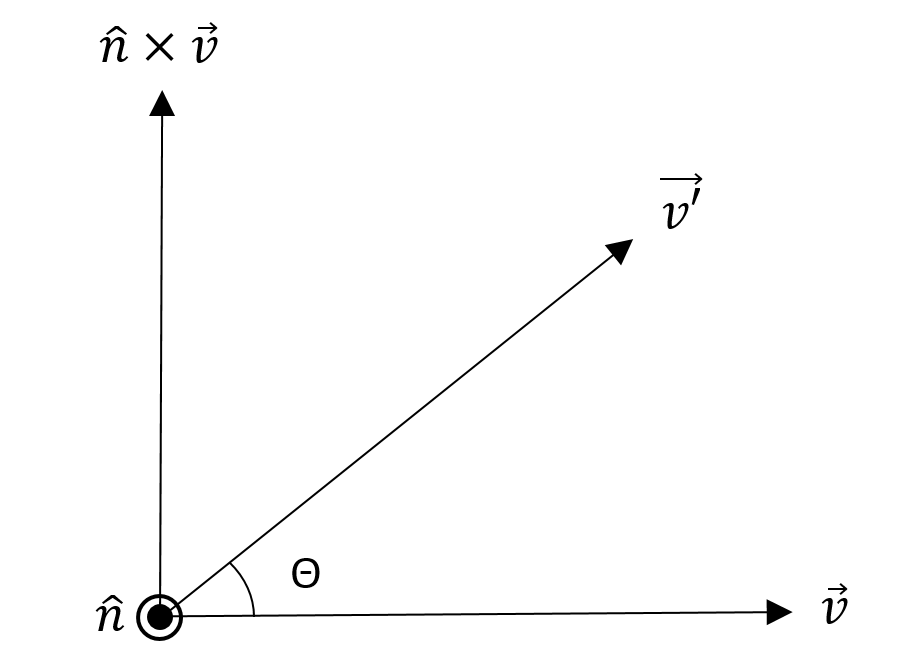
\includegraphics[scale=0.3]{nv.PNG}
\caption{Perpendicular Rotation}
\label{nv}
\end{figure}

Therefore, we can express $\vec{v}\,'$ as referred in figure \ref{nv}: 
$$
\boxed{
\vec{v}\,' = \cos(\theta)\vec{v} + \sin(\theta)(\hat{n}\wedge\vec{v})
}
$$
Let us write:
$$
v = (0,\vec{v}), \: v' = (0,\vec{v}\,'), \: n = (0,\hat{n})
$$
$$
nv = (-\hat{n}\cdot\vec{v}, \hat{n}\wedge\vec{v}) = \hat{n}\wedge\vec{v}
$$
$$
n^2 = -1
$$
Therefore, in quaternion notation, the equation becomes:
$$
v' = \cos(\theta)v + \sin(\theta)nv = \left(\cos(\theta) + \sin(\theta)n\right)v
$$
by rewriting this result as a quaternion exponential with the vector part equal to $\theta\hat{n}$:
$$
\boxed{
v' = e^{\theta n}v = ve^{-\theta n}
}
$$
So we can extract an important result for \textbf{normal} vectors $\hat{n}$, respectively quaternions $n = (0,\hat{n})$: 
$$
\boxed{
e^{\theta n} = \cos(\theta) + \sin(\theta)\hat{n} 
			 = \cos(\theta) + \sin(\theta)(n_xi + n_yj + n_zk)
}
$$

\subsection{General Case}
If $\vec{v}$ is no longer perpendicular to $\hat{n}$, $\vec{v}$ can be decomposed into:
$$
\vec{v} = \vec{v}_\parallel + \vec{v}_\perp
$$
where after a rotation, the only change is:
$$
\vec{v}\,' = \vec{v}_\parallel + \vec{v}_\perp\,'
$$
\subsubsection{3D Rotation with Vectors}
Therefore, from the special case:
$$
\vec{v}\,' = \vec{v}_\parallel + \cos(\theta)\vec{v}_\perp + \sin(\theta)(\hat{n}\wedge\vec{v}_\perp)
$$
with
$$
\hat{n}\wedge\vec{v} = \hat{n}\wedge(\vec{v}_\parallel + \vec{v}_\perp) = \hat{n}\wedge\vec{v}_\perp
$$
$$
\vec{v}_\perp = \vec{v} - \vec{v}_\parallel
$$
we can rewrite it as a function of $\vec{v}$ and $\vec{v}_\parallel$:
$$
\vec{v}\,' = (1-\cos(\theta))\vec{v}_\parallel + \cos(\theta)\vec{v} + sin(\theta)(\hat{n}\wedge\vec{v})
$$
With $\vec{v}_\parallel = (\vec{v}\cdot \hat{n})\hat{n}$, we obtain the \emph{Rodrigez Formula} for rotating any vector around any axis:
$$
\boxed{
\vec{v}\,' = (1-\cos(\theta))(\vec{v}\cdot \hat{n})\hat{n} + \cos(\theta)\vec{v} + \sin(\theta)(\hat{n}\wedge\vec{v})
}
$$

\subsubsection{3D Rotations with Quaternions}
By taking the notation:
$$
v = (0,\vec{v})
$$
From the special case, we can rewrite the general case as:
$$
v' = v_\parallel + v_\perp' = v_\parallel + e^{\theta n}v_\perp
$$
We need to observe the following properties (confirmed by applying the multiplication rule): 
$$
e^{\theta n}v_\perp = v_\perp e^{-\theta n} 
$$
$$ e^{\theta n}v_\parallel = v_\parallel e^{\theta n}
$$
Keeping these properties in mind, we can write:
\begin{equation*}
\begin{aligned}
v' &= v_\parallel + e^{\theta n}v_\perp \\
&= e^{\frac{\theta}{2}n}e^{-\frac{\theta}{2}n} v_\parallel + e^{\frac{\theta}{2}n}e^{\frac{\theta}{2}n} v_\perp \\
&= e^{\frac{\theta}{2}n} v_\parallel e^{-\frac{\theta}{2}n} + e^{\frac{\theta}{2}n} v_\perp e^{-\frac{\theta}{2}n} \\
&= e^{\frac{\theta}{2}n} (v_\parallel + v_\perp) e^{-\frac{\theta}{2}n} \\
&= e^{\frac{\theta}{2}n} v e^{-\frac{\theta}{2}n}
\end{aligned}
\end{equation*}

The compact form for rotation with quaternions is then given by: 
$$
\boxed{
v' = e^{\frac{\theta}{2}n} v e^{-\frac{\theta}{2}n}
}
$$
\begin{equation*}
\begin{aligned}
q &= e^{\frac{\theta}{2}n} &= \cos\left(\frac{\theta}{2}\right) + \sin\left(\frac{\theta}{2}\right)(n_xi + n_yj + n_zk) \\
q^* &= e^{-\frac{\theta}{2}n} &= \cos\left(\frac{\theta}{2}\right) - \sin\left(\frac{\theta}{2}\right)(n_xi + n_yj + n_zk)
\end{aligned}
\end{equation*}
$$
\boxed{v' = qvq^*}
$$

\newpage
\section{Summary}
$$
\boxed{
i^2 = j^2 = k^2 = ijk = -1
}
$$
\begin{center}
\begin{tabular}{c|ccc}
$\cdot\Rsh$ & i & j & k \\ 
\hline 
i & -1 & k & -j \\ 
j & -k & -1 & i \\ 
k & j & -i & -1 \\ 
\end{tabular} 
\end{center}
$$
\boxed{
q_1q_2 = (w_1w_2 - \vec{v_1}\cdot\vec{v_2}, w_2\vec{v_1} + w_1\vec{v_2} + \vec{v_1}\wedge\vec{v_2})
}
$$
$$
\boxed{
\vec{v}_1\cdot\vec{v}_2 = -\frac{1}{2}(v_1v_2 + v_2v_1)
}
$$
$$
\boxed{
\vec{v}_1\wedge\vec{v}_2 = \frac{1}{2}(v_1v_2 - v_2v_1)
}
$$
$$
\boxed{
e^q = e^{a + bi + cj + dk} = e^a\left(\cos(\Vert\vec{v}\Vert) + \frac{\sin(\Vert\vec{v}\Vert)}{\Vert\vec{v}\Vert}(bi + cj + dk)\right)
}
$$
$$
\boxed{
e^{\theta n} = \cos(\theta) + \sin(\theta)\hat{n} 
			 = \cos(\theta) + \sin(\theta)(n_xi + n_yj + n_zk)
}
$$
$$
\boxed{
\vec{v}\,' = (1-\cos(\theta))(\vec{v}\cdot \hat{n})\hat{n} + \cos(\theta)\vec{v} + \sin(\theta)(\hat{n}\wedge\vec{v})
}
$$
$$
\boxed{
v' = e^{\frac{\theta}{2}n} v e^{-\frac{\theta}{2}n}
}
$$
$$
\boxed{v' = qvq^*}
$$

\end{document}